\documentclass[a4paper, 11pt]{scrartcl}
\usepackage[utf8]{inputenc}
\usepackage[top = 2.5cm, bottom = 2cm, left = 2.5cm, right = 2.5cm]{geometry}
\usepackage[onehalfspacing]{setspace}
\usepackage{mathtools}
\usepackage{fontspec}
\usepackage{graphicx}
\usepackage[english]{babel}
\usepackage{enumerate}
\usepackage{tabularx}
\usepackage{booktabs}
\usepackage{hyperref}
\hypersetup{colorlinks = true, linkcolor = black, citecolor = blue, urlcolor = blue}
\usepackage{csquotes}
\usepackage[backend = biber, style = apa]{biblatex}
\addbibresource{../iris_literature.bib}


\title{IRIS model validation: Lessons learned}
\author{}
\date{\today}

\begin{document}
\maketitle
\tableofcontents


\newpage
\section{Motivation}
The IRIS model was validated with observation data from a sampling site near Regensburg. The aim of the model validation was to check how well the simulated model results match
with observed data. This includes the analysis of the influence of parameters for which we either found no clear values in the literature (e.g.\ for the activation rate) or
which change from year to year but are needed for initialisation such as the initial number of larvae or nymphs. In this context, we have also analysed the influence of the
beech mast which has an influence on the initial number of larvae which in turn has an influence on a possible second ``abundance peak'' of questing nymphs in a given year. For
this purpose, we have performed sensitivity analyses over a range of plausible values for these parameters and quantified the matching of the simulation results with the
observed data from the sampling site. Here, we present the results of this validation.


\section{Validation data}
For the validation we used a data set with monthly observations of nymphal ticks per $100 m^2$ of a 10-year period from a sampling site in Haselmühl where
\textit{Ixodes ricinus} ticks were collected using the flagging method~\parencite{Brugger.2017}. The time series with data between 2009 and 2018 was provided by
Gerhard Dobler\footnote{Bundeswehr Institute of Microbiology, Neuherbergstraße 11, 80937 Munich, Germany} via our cooperation partner Katharina
Brugger\footnote{Institute for Veterinary Public Health, University of Veterinary Medicine Vienna, Veterinärplatz 1, 1210 Vienna, Austria}. The observation data was also
used for model validation by~\textcite{Brugger.2017, Brugger.2018}.


\section{Evaluation criteria}
We use the root mean square error (RMSE) to quantify the differences of the simulated from the observed monthly nymphal densities. It was calculated for each of the 10 years of
the available validation data using the following formula:

\begin{equation}\label{eq:rmse}
RMSE_{year} = \sqrt{ \frac{1}{n} \sum_{i=1}^n (V_{sim}^i - V_{obs}^i)}
\end{equation}

with total number of monthly observations $n$, observed values $V_{obs}$ and simulated values $V_{sim}$ of a given year. A perfect fit corresponds to an RMSE value of 0, i.e.\
simulated and observed data match exactly. The higher an RMSE value the poorer is the matching. Months with missing data (NA-values) were not taken into account when
calculating the RMSE of a given year.

In order to evaluate the entire 10-year validation period, the annual RMSE values were added up and a total root mean square error $RMSE_{total}$ was calculated, hence
\begin{equation}\label{eq:total_rmse}
RMSE_{total} = \sum_{year=2009}^{2018} RMSE_{year}
\end{equation}


\section{Sensitivity Analyses}
We conducted sensitivity analyses to analyse the influence of the (1) initial number of larvae, (2) the initial number of nymphs and (3) the activation rate of the activity sub
model.

The initial number of larvae and nymphs at the beginning of a simulation run has an influence on the number of active nymphs throughout the year including the height of the
abundance peaks. Since we were interested in how the initial number of ticks controls the abundance peaks and since we didn't know the real initial values at the beginning of a
simulation, we were interested in the influence of these parameters. In this context, we also wanted analyse the influence of the beech mast process of our model. In
particular we wanted to find out whether the beech mast improves the matching of the model output with the real data. Since it affects the initial number of larvae, it
is also possible that this process can be neglected because the initial number of larvae can also be initialised directly\footnote{For details regarding the beech mast
see the ODD protocol of the IRIS model.}. Therefore, the sensitivity analyses were carried out with both the beech mast activated and deactivated.

The activation rate is an important model parameter. It is responsible for controlling the number of questing and inactive ticks in each time step. When microclimatic
conditions are suitable for questing, the number of questing ticks increases with a specific activation rate and the number of inactive ticks is reduced accordingly (and vice
versa)\footnote{For details regarding the activity sub model see the ODD protocol of the IRIS model.}. Since we did not find a value for the activation
rate in the literature, we estimated it through systematic variation within the presented sensitivity analyses.

We have carried out five sensitivity analyses:

\begin{enumerate}
\item[] \textbf{S1:} Equal number of larvae and nymphs, with beech mast activated
\item[] \textbf{S2:} Equal number of larvae and nymphs, without beech mast deactivated
\item[] \textbf{S3:} Larvae and nymphs individual variation, with beech mast activated
\item[] \textbf{S4:} Larvae and nymphs individual variation, without beech mast deactivated
\item[] \textbf{S5:} Higher share of initial number of Larvae, with beech mast activated
\end{enumerate}

In the first two sensitivity analyses (S1, S2), the initial number of larvae and nymphs was kept equal when varying these parameters within the sensitivity analysis (i.e.\ in
the for-loop). If, however, the beech mast model process was activated, the initial number of larvae was adjusted at the beginning of the simulation run, resulting in the actual
starting values being different. In the subsequent analyses (S3, S4), the number of larvae and nymphs was varied individually. At the beginning of a simulation run, the initial
numbers of larvae and nymphs could therefore differ considerably. An additional analysis (S5) was carried out to test the effect of the initial number of larvae being
significantly greater than the initial number of nymphs. The results are presented in the following sections.


\newpage
\subsection{S1: Equal number of larvae and nymphs, with beech mast activated}
In this sensitivity analysis, the following parameters were varied:


\begin{enumerate}
\item Initial number of nymphs: [1, 800, 1]
\item Initial number of larvae: = Initial number of nymphs
\item Activation rate: [0.016, 0.022, 0.001]
\end{enumerate}


\begin{figure}[h!]
\centering
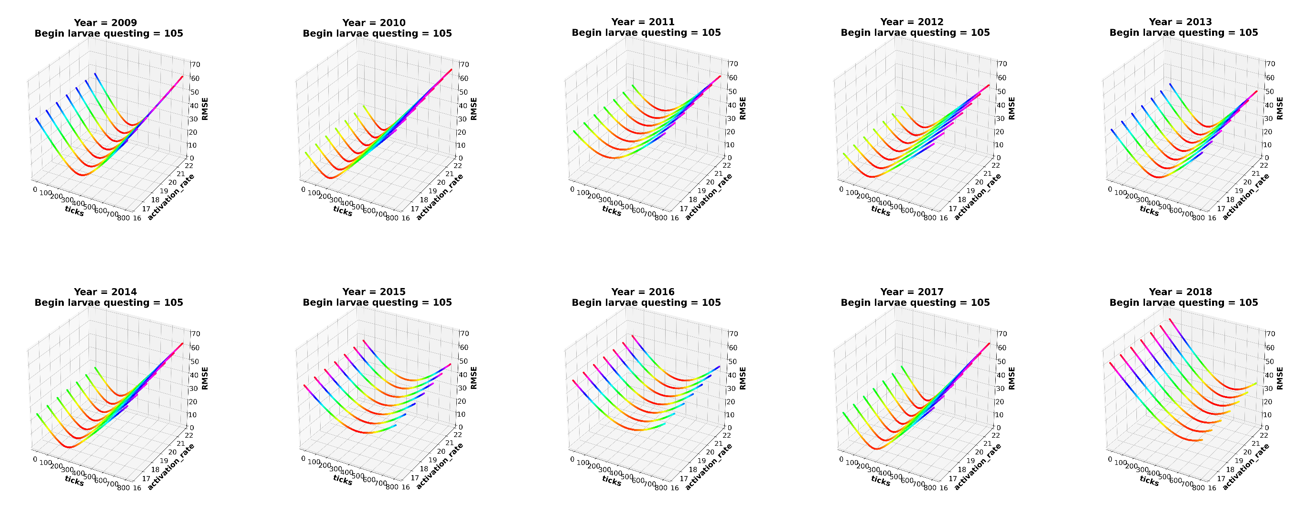
\includegraphics[width=1.0\textwidth]{figures/initial_ticks_with_beech_error.PNG}
\caption{initial ticks with beech error}
\label{fig:initial_ticks_with_beech_error}
\end{figure}

\begin{figure}[h!]
\centering
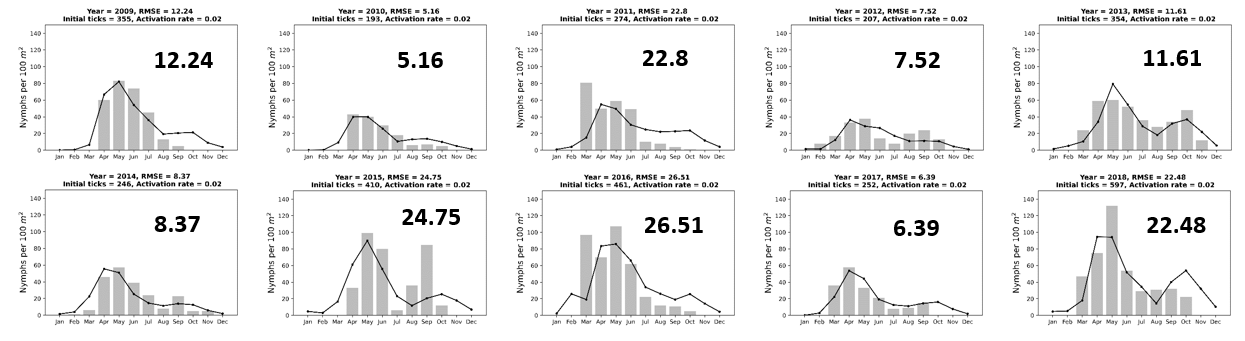
\includegraphics[width=1.0\textwidth]{figures/initial_ticks_with_beech.PNG}
\caption{initial ticks with beech}
\label{fig:initial_ticks_with_beech}
\end{figure}

The $RMSE_{total} = 147.85$
activation rate = 2.0 \%

\newpage
\subsection{S2: Equal number of larvae and nymphs, without beech mast deactivated}
RMSE = 154.89
activation rate = 2.1 \%

\begin{figure}[h!]
\centering
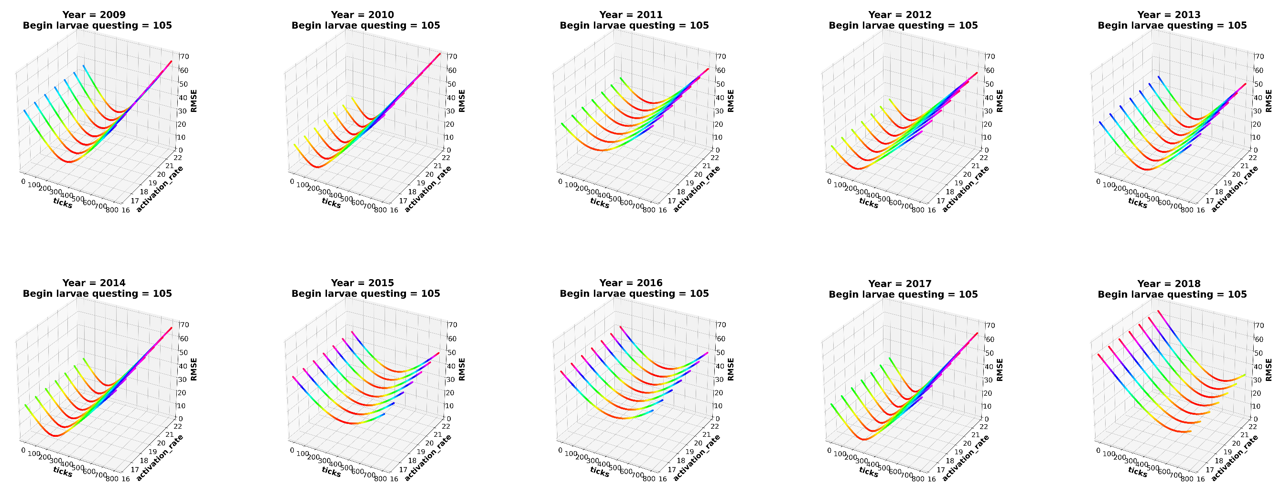
\includegraphics[width=1.0\textwidth]{figures/initial_ticks_without_beech_error.PNG}
\caption{initial ticks without beech error}
\label{fig:initial_ticks_without_beech_error}
\end{figure}

\begin{figure}[h!]
\centering
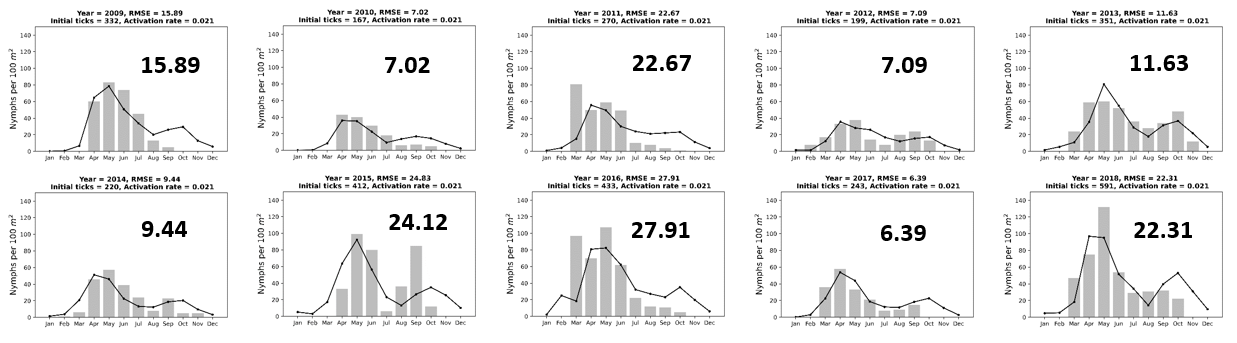
\includegraphics[width=1.0\textwidth]{figures/initial_ticks_without_beech.PNG}
\caption{initial ticks without beech}
\label{fig:initial_ticks_without_beech}
\end{figure}



\newpage
\subsection{S3: Larvae and nymphs individual variation, with beech mast activated}


\begin{table}[h!]
\caption{Input parameters}
\label{tab:independent_initial_ticks_params}
\begin{tabularx}{\textwidth}{lccc}
\toprule
\textbf{Parameter} 	& \textbf{Start value} & \textbf{End value} & \textbf{Step size} \\
\midrule
initialLarvae   	& 0 		& 800  		& 10 \\
initialNymphs   	& 10   		& 800	 	& 10 \\
Activation rate     & 0.016     & 0.022   	& 0.001 \\
\bottomrule
\end{tabularx}
\end{table}


\begin{figure}[h!]
\centering
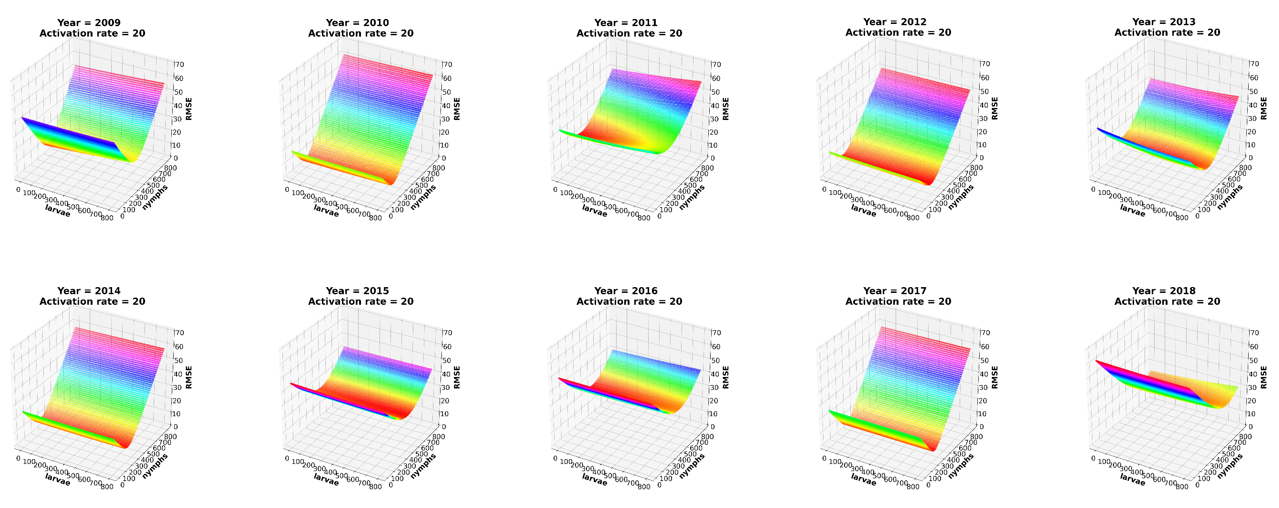
\includegraphics[width=1.0\textwidth]{figures/independent_initial_ticks_with_beech_error.PNG}
\caption{independent initial ticks with beech error}
\label{fig:independent_initial_ticks_with_beech_error}
\end{figure}

\begin{figure}[h!]
\centering
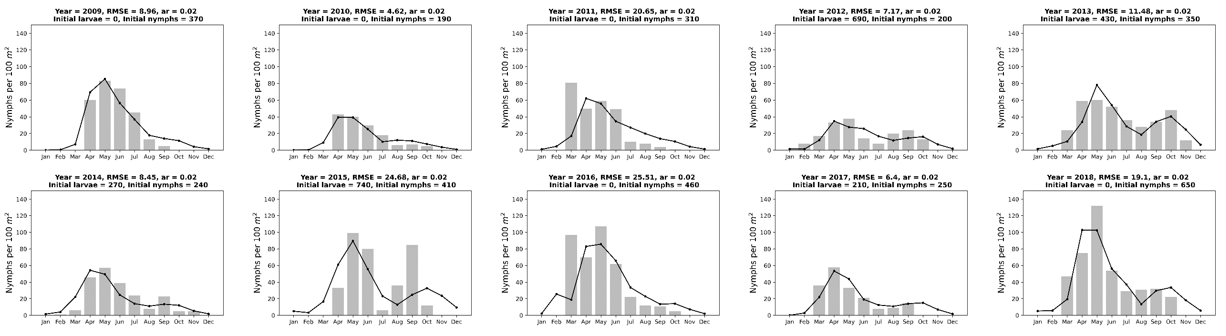
\includegraphics[width=1.0\textwidth]{figures/independent_initial_ticks_with_beech.PNG}
\caption{independent initial ticks with beech}
\label{fig:independent_initial_ticks_with_beech}
\end{figure}

Summe RMSE = 137.13
activation rate = 2.0 \%

\newpage
\subsection{S4: Larvae and nymphs individual variation, without beech mast deactivated}


\begin{figure}[h!]
\centering
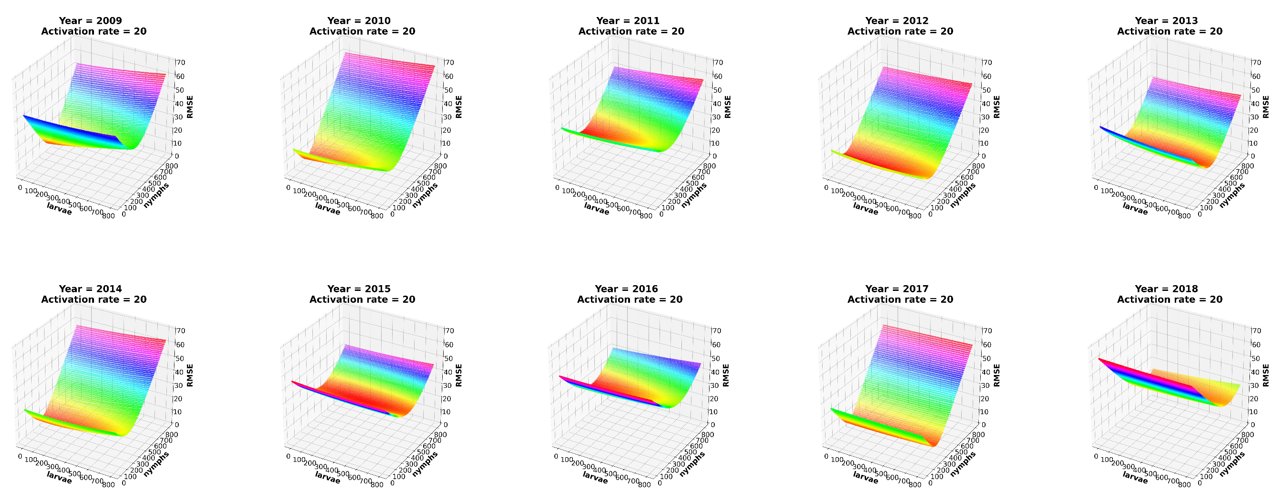
\includegraphics[width=1.0\textwidth]{figures/independent_initial_ticks_without_beech_error.PNG}
\caption{independent initial ticks without beech error}
\label{fig:independent_initial_ticks_without_beech_error}
\end{figure}

\begin{figure}[h!]
\centering
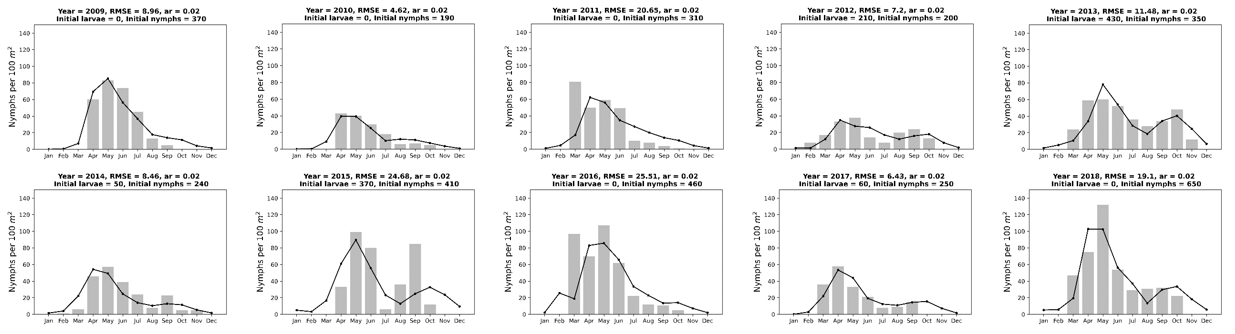
\includegraphics[width=1.0\textwidth]{figures/independent_initial_ticks_without_beech.PNG}
\caption{independent initial ticks without beech}
\label{fig:independent_initial_ticks_without_beech}
\end{figure}

Summe RMSE = 137.17
activation rate = 2.0 \%


\subsection{S5: Higher share of initial number of Larvae, with beech mast activated}
4 x initial Nymphs (with beech mast)
RMSE = 192.13
activation rate = 1.9 \%

Total RMSE with optimal parameter combination higher than in the other sensitivity analyses. But


\section{Lessons Learned}

% Hier Übersichtstabelle einfügen

In summary we have learned that

\begin{enumerate}
\item the validation results show a good overall correspondence of our simulation output with the observed data~\parencite{Brugger.2017}.
\item the matching of simulated in terms of RMSE was (very) good in some years (RMSE < 10).
\item some years were difficult to capture by our model: 2011, 2015, 2016, 2018 (with RMSE > 20).
\item the best fit with observed data was achieved when activation rate was 0.02 (1x 0.019,  3x 0.02,  1x 0.021).
\item the initial number of larva had a very minor influence when the initial number of larvae and nymphs were varied independently.
\item with individual variation of initial larvae and nymphs, the influence of the beech mast had little effect.
\item the variation with the same number of initial larvae and nymphs was improved by the beech mast.
\item a strong increase of initial larvae led to an increase of the second abundance peak, however the overall matching got worse.
\end{enumerate}


\printbibliography[heading = bibintoc, title = {Bibliography}]

\end{document}